%!TEX TS-program = xelatex
% vim: set fenc=utf-8

% -*- coding: UTF-8; -*-
%!TEX encoding = UTF-8
\documentclass[twoside]{CUGThesis}

\title{基于U-Net网络的遥感图像语义分割} %论文题目
\author{郭子睿} %作者姓名
\date{\today} %日期,默认当日
\school{计算机学院} %院系名称
\classnum{计算机科学与技术} %专业
\stunum {20151003952} %学号
\instructorone{李显巨} %指导教师1姓名
\instructoronelevel{副教授}

\usepackage{makecell}
\usepackage{multicol}
\usepackage{multirow}
\usepackage{hyperref}

\begin{document}
\maketitle
\makestatement

\begin{cnabstract}{U-Net;语义分割;遥感图像}
	在计算机视觉中,图像分割是将数字图像细分为多个图像子区域的过程。分割的目标是将图像的表示更改为更有意义且更易于分析的内容。更确切地说,图像分割是对图像中的每个像素打上标签的过程,相同标签的像素有某些相似的视觉特征。

	遥感图像分割主要目的是在遥感图像中定位诸如道路、房屋、林业资源的物体以达到统计国土资源或进行土地规划的目的。遥感图像尺寸巨大,内容复杂。传统遥感图像分割主要依赖人工标注,工作量大。因此,开发一种自动遥感图像分割算法是十分有必要的。

	本文尝试使用U-Net对遥感图像进行语义分割,并对使用U-Net进行遥感图像语义分割的可行性做出了评估。
\end{cnabstract}

\begin{enabstract}{U-Net; Semantic Segmentation; Remote Sensing Image}
	In the field of computer vision,image segmentation is refered to partitioning a digital image into multiple areas. The aim of segmentation is to simplify and change the representation of an image into something that is more meaningful and easier to analyze.More specificly, image segmentation is the process of assigning a label to every pixel in an image such that pixels with the same label share certain characteristics.

	The main purpose of remote sensing image segmentation is to locate objects such as roads, houses, and forestry resources in remote sensing images to achieve the purpose of statistical land resources or land planning. Remote sensing images are large in size and complex in content. Traditional remote sensing image segmentation mainly relies on manual labeling and has a large workload. Therefore, it is very necessary to develop an automatic remote sensing image segmentation algorithm.

	This paper attempts to use Semantic Separation of Remote Sensing Images by U-Net and evaluates the feasibility of using U-Net for semantic segmentation of remote sensing images.
\end{enabstract}

\makeToc

%---------------------------------------------开始正文---------------------------------------------
\begin{spacing}{2}
    \section{先行研究}
\end{spacing}
图像分割问题从计算机被用于处理的那天开始就是一个核心问题。通过总结之前的算法,我们也许可以提出一些新的方法。
\subsection{图像分割技术的历史}
图像分割技术的演进历史大概可以分为基于图论的方法、基于像素聚类的方法和基于深度语义的方法三段。其中基于图论的方法和基于像素聚类的方法都被视为传统图像分割技术。而最新的图像分割算法基本上都是基于语义的分割算法。

基于图论的方法把图像分割问题与图的最小割问题相关联,分割的原则是使划分后的子图在内部保持相似度最大,而子图之间的相似度保持最小。

机器学习中的聚类算法如K-means、谱聚类等也应用于图像分割问题。通常的思路是利用诸如颜色、亮度、纹理等特征对像素点进行聚类。

传统的图像分割算法中主要是基于底层的特征,而基于语义的分割算法可以基于图像中高层内容信息对图像进行分割。因此语义分割算法在对结构复杂,内部差异性大的物体进行分割的时候表现较传统图像分割技术好。

遥感图像中,既有道路、森林等有相对固定的纹理的物体,也有建筑、港口等较为复杂的物体。对于简单的物体的分割,传统的基于图论的方法和基于像素聚类的方法可能会对我们有所启示;而那些复杂的物体基于语义图像分割技术可能会有更好的效果。
\subsection{深度学习与图像分割}
作为深度学习中一个常见的任务,基于语义的图像分割技术已有了长足的发展。现如今,一个通用的框架已确定,那就是在前端使用神经网络对特征进行提取,后端再利用马尔可夫随机场等优化方案对前端的输出进行优化,输出分割图片。

2015年之前,人工神经网络在图像分类任务上表现良好。但在图像语义分割任务上的表现差强人意。2015年,加州大学伯克利分校的 Long 等人的论文\cite{long2015fully}发表。自此,一大批受全卷积网络启发的神经网络开始涌现,人工神经网络开始广泛应用于图像语义分割任务。
\subsubsection {全卷积网络与语义分割网络设计准则}
作为人工神经网络应用于图像语义分割的开山之作,全卷积网络现已有了广义和狭义两种定义。狭义上的全卷积网络指 Long 等人的论文\cite{long2015fully}中提出的用于图像语义分割的神经网络。而广义的全卷积网络则是指一类用全卷积层替代全连接层的神经网络。下面的全卷积网络指的是狭义上的全卷积网络。
\cite{long2015fully}为我们提供了三个语义分割网络设计准则:
\begin{enumerate}
    \item 用全卷积层替换全连接层来保留位置信息;
    \item 通过上采样还原因池化操作造成的位置信息损失;
    \item 利用深监督或跳跃连接结合浅层信息,优化输出。
\end{enumerate}
下面我对这三个准则进行阐述。
\paragraph{全连接层与全卷积层}
我们从人工神经网络的应用历史可以知道,人工神经网络最开始用于图像分类。一个经典的用于图像分类的网络,如\cite{krizhevsky2012imagenet}中提出的AlexNet,通过在卷积层之后连接上若干个全连接层,将卷积层提取的特征图映射成一个特征向量。这个特征向量在经过归一化处理之后,可以用来表示图像属于每一类的概率,进而达到对图像分类的目的。

图像分割任务也可以被视作一个分类任务,即通过将像素分到不同的类别达到分割的效果。全连接层将二维的图像压缩成了一位的特征向量从而丢失了定位像素的空间信息。因此在全卷积网络中,传统的用于图像分类的网络的全连接层被替换成了全卷积层。

在\cite{long2015fully}中,Long 等人对有广泛应用的分类网络 VGG16\cite{simonyan2014very} 进行改造,去掉了最后的全连接层,加上了全卷积层。丢弃全卷积层作为重要的用于图像分割的神经网络设计准则被广泛接受。不论是用于场景解析的 PSPNet\cite{zhao2017pyramid} 和 SegNet\cite{badrinarayanan2017segnet} 还是用于医疗图像分割的 U-Net\cite{ronneberger2015u} 都使用全卷积层来替换全连接层。


\paragraph{池化层与上采样}
池化层可以增加输入图像对一些小扰动的鲁棒性,更重要的是池化层增大了感受野,这对提取高层语义信息十分重要。但池化层与全连接层一样,对保留像素的位置信息是很不利的。因此如何恢复在池化层中丢失的位置信息是语义分割网络的重要议题。

在\cite{long2015fully}中,Long 等人提出通过对输入数据进行上采样恢复到输入图像的大小来补充位置信息。这篇论文中上采样不是使用简单的双线性插值,而是通过学习实现插值操作。然而,由于在池化操作中丢失部分信息,使得即使加上反卷积层的上采样操作也会产生粗糙的分割图。

除插值操作之外,其他受\cite{long2015fully}启发的论文中也提出了其他对抗池化层的方法,其中主流的思路有以下两种:

\begin{enumerate}
    \item 编码器-解码器结构
    
    编码器-解码器结构是一种常见的恢复位置信息的方法。比较著名的网络有SegNet\cite{badrinarayanan2017segnet}和下面将要使用的U-Net\cite{ronneberger2015u}。编码器中,使用池化层减小输入数据的空间维度;解码器则通过反卷积层来增大空间维度。
    \item 空洞卷积
    
    使用空洞卷积来替代池化层。空洞卷积可以在不降低空间维度的前提下增大感受野。使用空洞卷积的有DeepLab\cite{chen2014semantic}系列网络。但使用空洞卷积计算成本较编码器-解码器方案高,因此不适用于图像巨大的遥感图像处理。
\end{enumerate}
\paragraph{跳跃连接与深监督}
使用神经网络提取的特征,在浅层是简单的图像特征,如边界、颜色等。而深层由于感受野增大,我们可以提取更抽象的特征。为了获得更精确的语义分割结果,我们需要结合浅层语义信息。

上采样之后的结果还是十分粗糙。在\cite{long2015fully}中,Long等人将不同池化层的结果进行上采样之后进行加操作(summation)来优化输出。这种利用不同深度特征来优化输出的思路在其后的网络中也有迹可寻。

在\cite{ronneberger2015u}中,作者则是将上采样中大小差不多的层与下采样中不同深度的池化层进行叠操作(concatenation)之后再进行卷积操作。这样做的好处是在通过上采样恢复时可以利用浅层信息,从而达到更精准的分割效果。

深监督网络\cite{lee2015deeply}可以提高隐藏层学习过程的直接性和透明度。深监督网络的核心思想是为隐藏层提供集成的直接监督层,而不是仅在输出层提供监督。通过为每个隐藏层引入伴随目标函数来提供这种集成的直接隐藏层监督;这些伴随目标函数可以被视为学习过程中的附加(软)约束。

引入深监督的语义分割网络有HEDNet\cite{xie2015holistically}。虽然这个网络是用于边缘检测,但是作者将边缘检测看做是一个图像分割问题:即将图像分割为边缘和非边缘两类。该网络与\cite{long2015fully}一样改装了VGG系列网络。与\cite{long2015fully}不同的是,它在VGG网络的各个隐层输出损失函数而非\cite{long2015fully}那样进行加操作。

\cite{lee2015deeply}与\cite{long2015fully}这两种非编码器-解码器结构的网络采用了两种不同的利用浅层语义信息的方式。可以说跳跃连接和深监督是利用浅层语义信息的两种思路。
\begin{spacing}{2}
    \section{研究方法}
\end{spacing}
U-Net首次出现在一次医疗图像分割赛事中。U-Net基于全卷积网路,使用对称结构并且在小数据集表现优异。同时,由于医疗影像的特殊性,作者在论文中特别提到了对于像医疗影像这样的尺寸巨大图像的特殊处理过程。

遥感图像和医疗影像的共同之处在于,数据集小、尺寸巨大。可以说,应用在医疗影像上的U-Net为我们提供了对遥感图像进行分割的重要思路。
\subsection{数据集选择及处理}
这次选择的数据集是Inria Aerial Image Labeling Dataset\cite{maggiori2017dataset}。数据集的图片大小为$5000\times 5000$,共计180组360张3通道遥感图像。样例如图\ref{Fig:sample_dataset}。

\begin{figure}[!t]
		\centering
		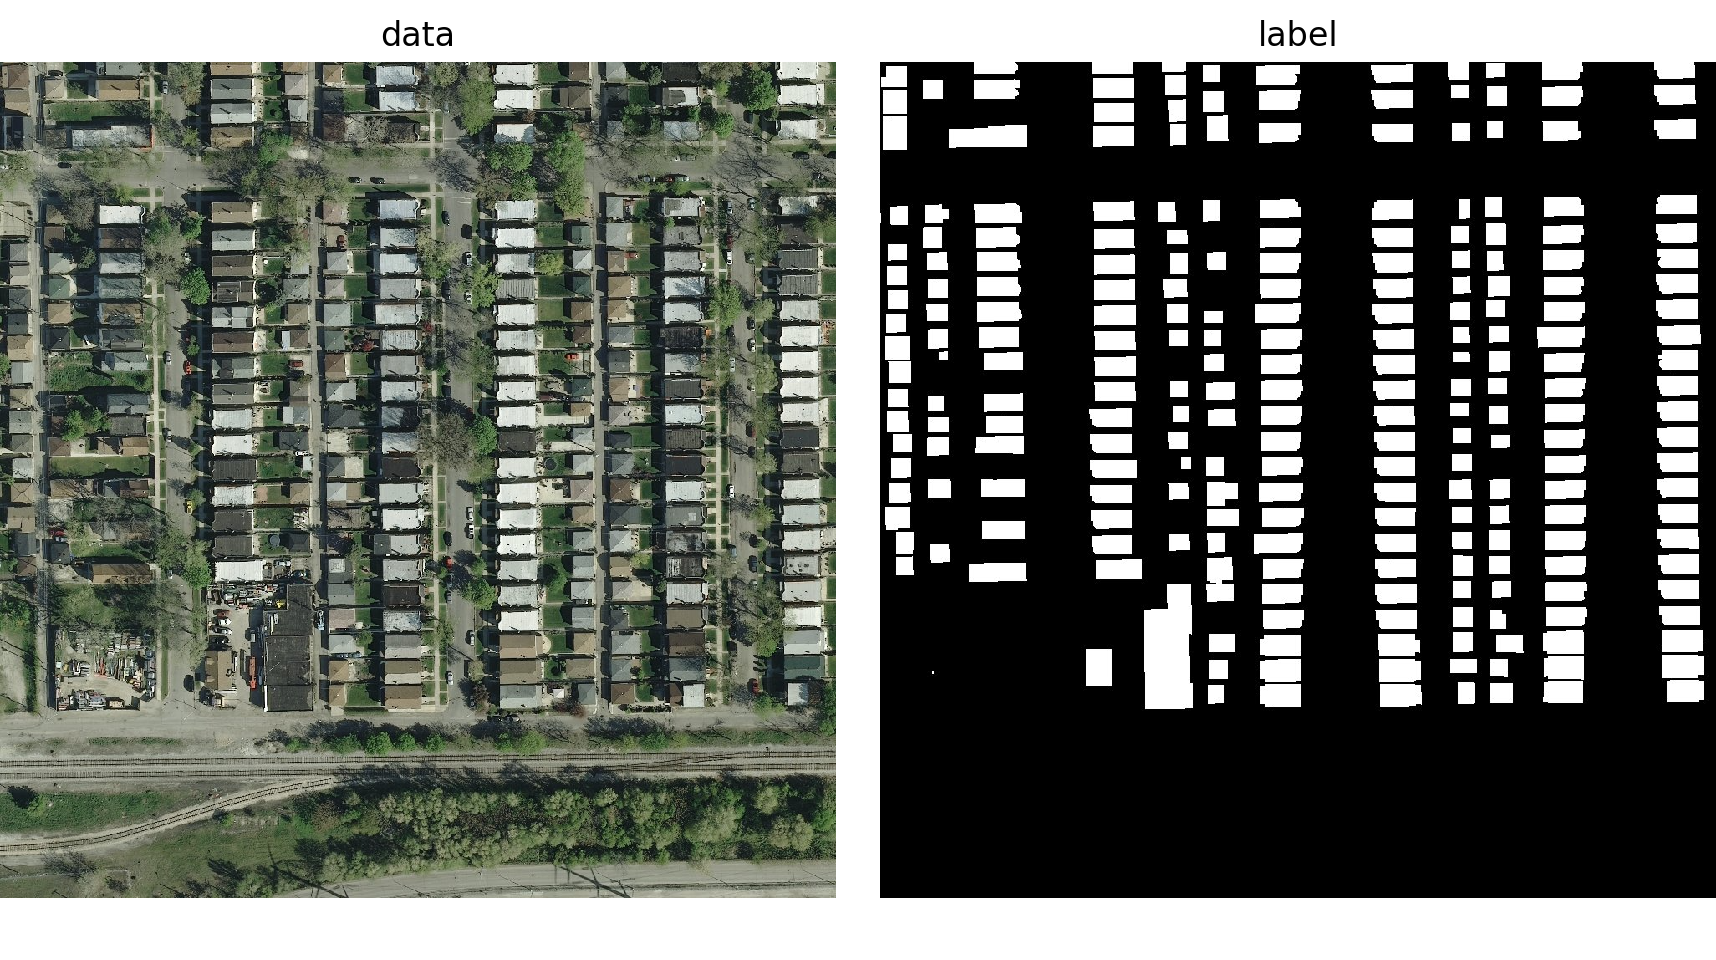
\includegraphics[width=1\textwidth]{Figures/sample_dataset.png}
		\caption{数据集样例图}
		\label{Fig:sample_dataset}
\end{figure}

由于显存限制,经过测试,$500\times 500$左右大小的图片一次只能只能训练一张。如果每次只训练一张的话,会陷入局部最优解。因此将图片切割为$250\times 250$左右大小的图片,mini batch size 大小可以设置为4。

由于池化核的大小为$2\times 2$,因此输入图片的大小最好是2的整次方。最终确定将图片切割为$256\times 256$。原图尺寸大小为$5000\times 5000$,因此将原图调整大小至$4864\times 4864$大小之后再进行分割。这样共得到了64980张图像。由于数据集本身已经够大,因此不再做数据拓展。
\subsection{图像处理流程设计}
\subsubsection{网络结构}
初始的U-Net网络结构如图\ref{Fig:unet_construction}所示。

网络分为收缩路径和扩张路径两部分。在收缩路径中,进行两次卷积核大小为$3\times 3$的卷积之后再进行$2\times 2$的最大池化。在扩张路径中将收缩路径中的卷积层拼接之后再进行两次大小为$3\times 3$的卷积。之后再进行反卷积慢慢恢复到原图像大小。

论文\cite{ronneberger2015u}中使用valid卷积方式。但是经过计算,$256\times 256$大小的图片在通过U-Net网络后,输出图片大小为$68\times 68$,与原图像大小相差太大,因此在这里选用same卷积方式,这样输出图片大小仍为$256\times 256$。除此之外没有对U-Net做更多结构上的修改。
\begin{figure}[!t]
    \centering
    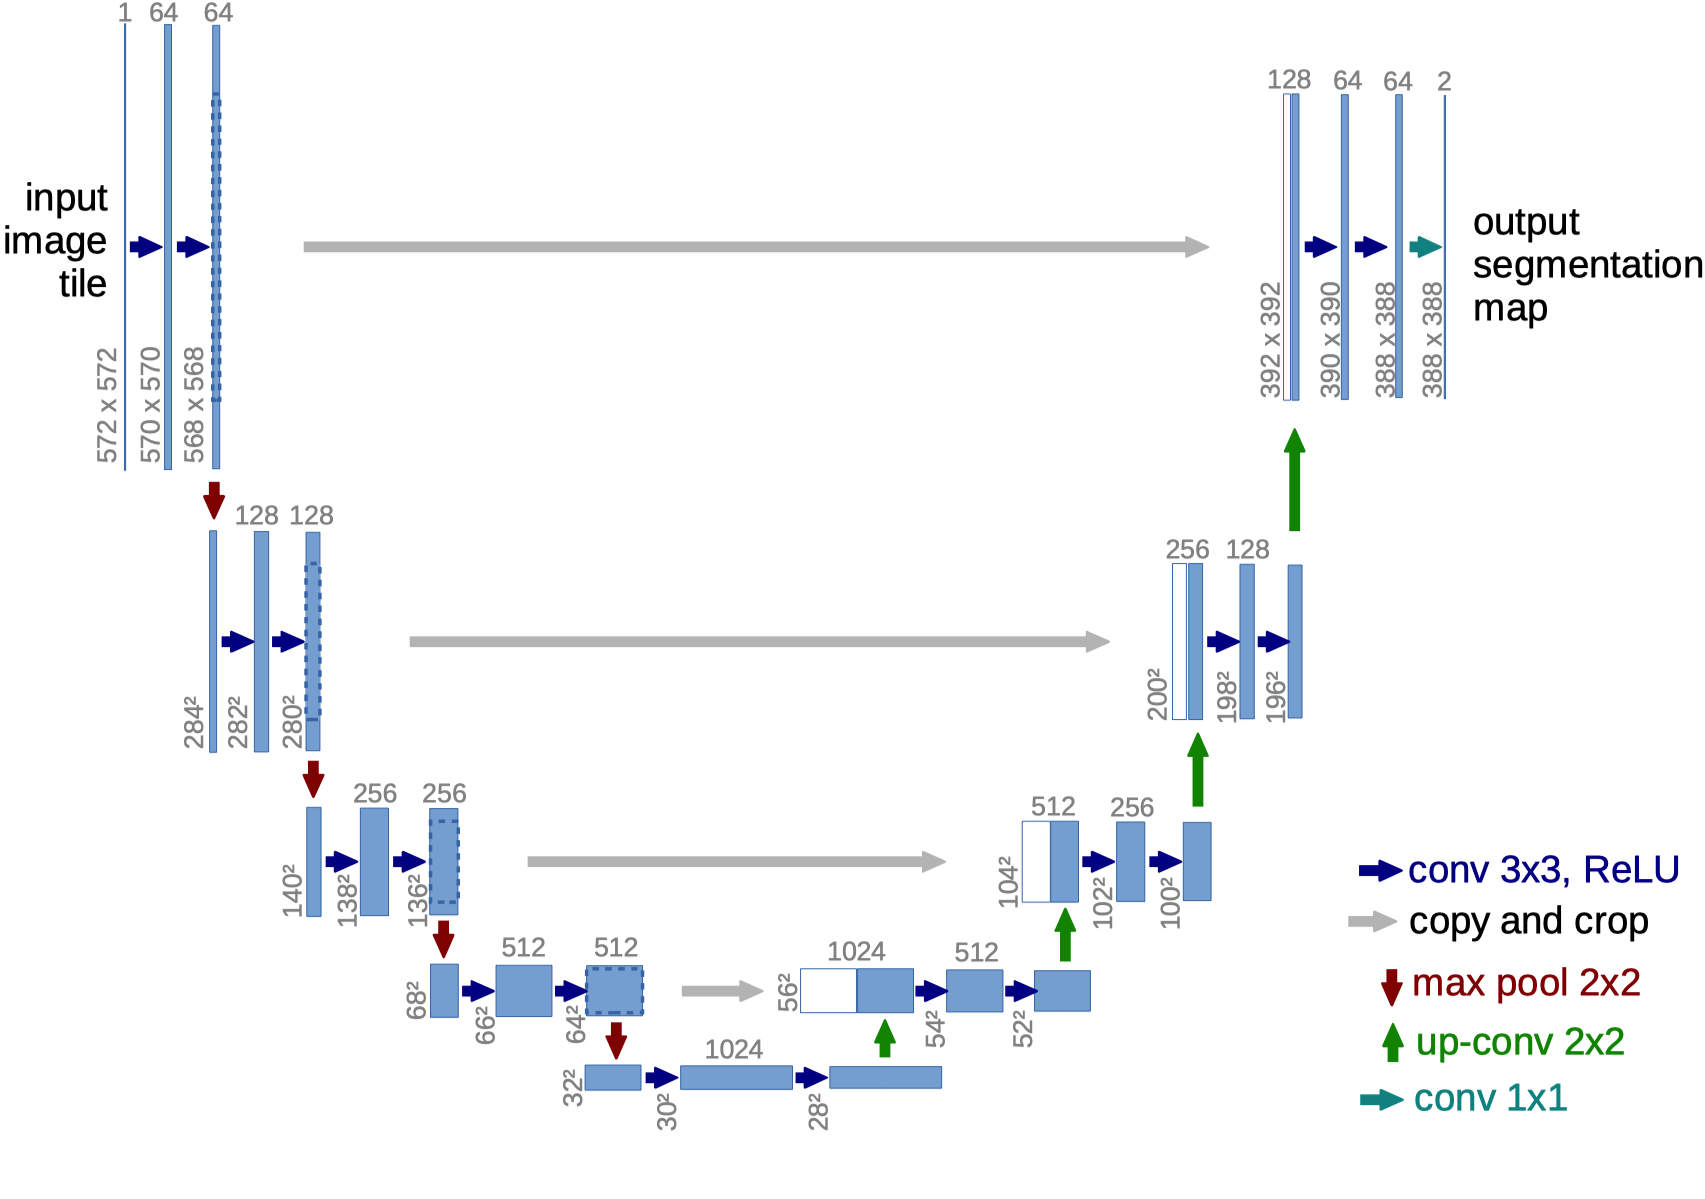
\includegraphics[width=1\textwidth]{Figures/unet_construction.png}
    \caption{U-Net网络结构(来源\cite{ronneberger2015u})}
    \label{Fig:unet_construction}
\end{figure}
\subsubsection{实验后处理}
通过之后的损失函数中权重的不同,训练出几个参数不同的神经网络。将同一张图通过不同的神经网络之后得到的输出图进行像素级或操作,得到融合的生成图。再对得到输出图之后对图像进行形态学处理,去除小面积空洞图和小面积误报区。
% https://blog.csdn.net/traumland/article/details/51419963
考虑到房屋多为多边形,因此使用霍夫变换检测出输出图中的多边形并标注为房屋。

在之前的论文中有人使用条件随机场对生成的图片做更精准的切分,这里时间有限就没有做这种尝试。
\subsection{损失设计}
原始的U-Net网络论文中使用的是交叉熵加上一些正则化项。除了交叉熵之外,此次实验还设计另外两种损失函数,将在之后的实验中做出对比。

在下面这三种损失函数中,都先对卷积网络输出图像做了soft-max计算:
\begin{equation}\label{softmax}
p_k(x)=\exp(\frac{a_k(x)}{\sum\limits_{k'=1}^K \ \exp(a_{k'}(x))})
\end{equation}

公式\ref{softmax}中$K$是分割类别数,$k\in K$。具体到这个数据集来说,类别分为建筑和非建筑,因此$K=2$。

$\mathbb{Z}^2$为全体像素集合,$x\in \mathbb{Z}^2$。$a_k(x)$即在$x$处类别$k$的取值。
\subsubsection{带权重的交叉熵}
\begin{equation}\label{entropy}
E=\sum_{x\in \Omega}\ w(x)\cdot \log(p_{l(x)}(x))
\end{equation}

公式\ref{entropy}中$l: \Omega\rightarrow\{1,\cdots,K\}$是每个像素点真正的类别;$w: \Omega\rightarrow\mathbb{R}$是权重。该权重将取不同值,在训练过程中进行比较。
\subsubsection{类别平衡交叉熵}
\begin{equation}\label{class_balanced_cross_entropy}
    l=-\beta\cdot \sum\limits_{j\in Y_+}\ \log\ \Pr(y_j=1|X)-(1-\beta)\cdot \sum\limits_{j\in Y_-}\ \log\ \Pr(y_j=0|X)
\end{equation}

在\cite{xie2015holistically}中提出了一种被称为类别平衡交叉熵函数的方法计算损失。因为边缘像素的数量远远小于非边缘像素的数量,因此在训练时容易陷入向全取非边缘像素方向的局部最优。在遥感图像中,被标记为房屋的像素与非房屋的像素数量也不是十分均衡的,因此在这里尝试使用类比平衡交叉熵,防止陷入局部最优解。

公式\ref{class_balanced_cross_entropy}中引入了一个像素级的类别平衡权重$\beta$,其值是被标记为建筑的像素占所有像素的比值。这实际上也是一种带权重的交叉熵,只不过该交叉熵的权重取得是两种标签的比值。


\begin{spacing}{2}
    \section{实验}
\end{spacing}
\subsection{网络初始化设计}
使用Adam Optimizer,经过初步实验,学习率定为$1^{-5}$,并使用指数衰减学习率,衰减率设为0.95。卷积核使用Xavier初始化方法。

%---------------------------------------------  致谢  ---------------------------------------------
\begin{spacing}{2}
	\section*{致谢}
	Send my love to everyone.
\end{spacing}
\phantomsection
\addcontentsline{toc}{section}{致谢}

\clearpage
%---------------------------------------------参考文献---------------------------------------------

\bibliography{Bibs/mybib}
\phantomsection
\addcontentsline{toc}{section}{参考文献}

\end{document}